% Chapter 2

\begin{savequote}[\quotewidth]
$PV \ne nRT$
\qauthor{The ideal gas law does not apply to supercritical fluids.}
\end{savequote}

\chapter{Introduction: Carbon dioxide and chromatography} % Main chapter title

\label{Chapter2} % Change X to a consecutive number; for referencing this chapter elsewhere, use \ref{ChapterX}


%----------------------------------------------------------------------------------------
%	SECTION 1
%----------------------------------------------------------------------------------------

\section{The chemical industry}

Industrialized societies depend on chemicals. (In this discussion I define
chemicals as pure substances that are produced by industry for industry.)
Chemicals might be used in the processing of products, or blended with other
chemicals in formulations that might be sold to users as products. In a familiar
example, sugar is a chemical produced by the sugar industry from sugar cane or sugar beet.
It is a pure substance (sucrose) that is mostly used in the industry as an
ingredient for processed food. Other uses of sugar include coatings for
medication, and feedstock for engineered micro-organisms that produce pharmaceuticals. (Sugar is a
rare example of a chemical that is also sold to consumers.)
 
The chemical industry produces a huge variety of products, from compounds as as
simple as hydrochloric acid to compound as sophisticated as cyanocobalamin
(Figure \ref{fig:vitb12}). All of these chemicals help produce the products
indispensable to industrialized societies. Nevertheless, the chemical industry
is not held in high regard by people outside the industry. A part of this
negative perception comes from the chemical industry's reputation for fatal
accidents and pollution \autocite{Gumm2015}.

\begin{figure}
\centering
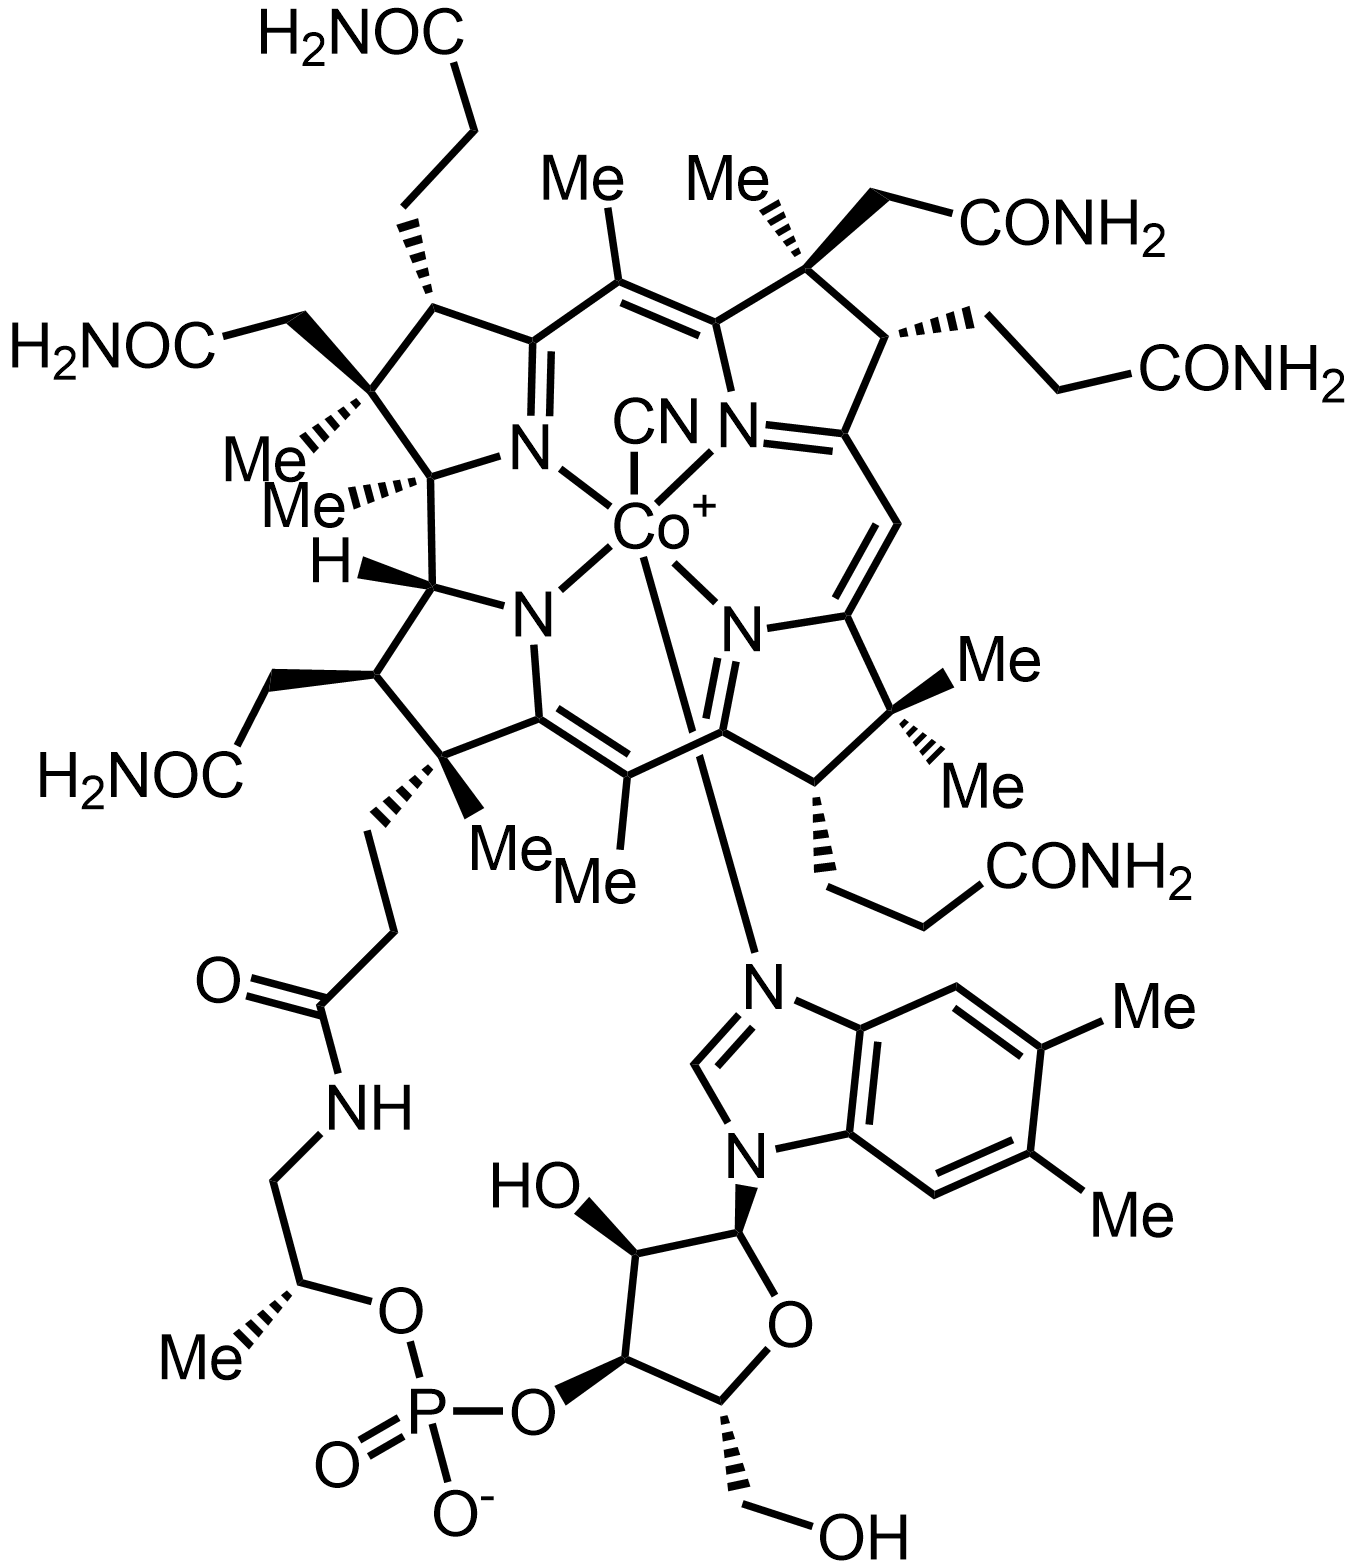
\includegraphics[width=\textwidth]{Figures/Cyanocobalamin-b12.png}
\decoRule
\caption[Cyanocobalamin]{The chemical structure of cyanocobalamin, a form of vitamin B12. This compound is produced on the tonne scale by the chemical industry.}
\label{fig:vitb12}
\end{figure}

The list of incidents is long and examples easily spring to mind: In 1984 a leak
at a chemical plant in Bhopal, India, caused the death of thousands of people
and the injury of thousands more \autocite{Varma2005}.
Stratospheric ozone is struggling to recover from depletion caused by the
reckless emissions of chlorofluorocarbons \autocite{Ball2018}. Plastics
microparticles are now found everywhere in the oceans \autocite{Woodall2014},
and the pesticide DDT is found in the breast milk of Inuit mothers
\autocite{Gibson2016}.

The chemical industry is also a prodigious producer of greenhouse gases. Apart
from the carbon dioxide emitted by the production of the energy that power
chemical processes, some chemical processes emit carbon dioxide as a waste
product. Most notable of these is the reduction of atmospheric nitrogen as the
first step in the production of nitrogen fertilizers. Of all the greenhouse
gases monitored by the IPCC, only carbon dioxide, methane and nitrous oxide are
found in nature: the others are exclusively products of the chemical industry
\autocite{IPCC2014}.

No chemical has ever jumped out of a lab, multiplied uncontrollably, and spread
into the environment to poison or pollute: they have all been introduced into
the environment by human ignorance, negligence, or recklessness. All chemicals
behave well when used in properly controlled environments, but human actions can
let them escape and damage and pollute. But while we try to solve the
intractable problem of human behaviour, we as chemists cannot just lay blame: we
must pay attention to the intrinsic safety of chemicals and chemical processes.
 
%-----------------------------------
%	SUBSECTION 1
%-----------------------------------
\subsection{``Green chemistry''}
\label{sec:GreenChemistry}
The date of the birth environmental movement is conventionally set to 1962, when
the biologist Rachel Carson published the book \textit{Silent Spring}, which
pointed out the destruction of nature by the unrestricted use of pesticides, and
the dangers of overuse \autocite{Carson1962}. This was a direct imputation of
the chemical industry, because the pesticide products contained many chemicals.

Chemists are human, and the realization uncontrolled that chemicals can have
detrimental effects lead at least some chemists to reflect on their own work.
This has given rise to the concept of \textit{green chemistry}. Although the
term has no rigorous definition or quantitative measure \autocite{Linthorst2010},
a set of 12 principles or guidelines are proposed:

\begin{enumerate}
  \item \label{itm:waste}It is better to prevent waste than to treat or clean up waste after it is formed.
  
  \item \label{itm:incorporation}Synthetic methods should be designed to maximize the incorporation of
  all materials used in the process into the final product.
  
  \item \label{itm:toxicity}Wherever practicable, synthetic methodologies should be designed to use
  and generate substances that possess little or no toxicity to human health and
  the environment.
  
  \item \label{itm:efficacy}Chemical products should be designed to preserve efficacy of function
  while reducing toxicity.
  
  \item \label{itm:aux}The use of auxiliary substances (\textit{e.g.} solvents, separation agents, etc.)
  should be made unnecessary wherever possible and innocuous when used.
  
  \item \label{itm:energy}Energy requirements should be recognized for their environmental and
  economic impacts and should be minimized. Synthetic methods should be
  conducted at ambient temperature and pressure.
  
  \item \label{itm:renewable}A raw material or feedstock should be renewable
  rather than depleting wherever technically and economically practicable.
  
  \item \label{itm:derivatization}Unnecessary derivatization (blocking group, protection/deprotection,
  temporary modification of physical/chemical processes) should be avoided
  whenever possible.
  
  \item \label{itm:catalysts}Catalytic reagents (as selective as possible) are superior to
  stoichiometric reagents.
  
  \item \label{itm:persistence}Chemical products should be designed so that at the end of their
  function they do not persist in the environment and break down into innocuous
  degradation products.
  
  \item \label{itm:monitoring}Analytical methodologies need to be further developed to allow for
  real-time, in process monitoring and control prior to the formation of
  hazardous substances.
  
  \item \label{itm:safe}Substances and the form of a substance used in a chemical process should
  be chosen so as to minimize the potential for chemical accidents, including
  releases, explosions, and fires.

\end{enumerate}

While these guidelines are clearly written with synthetic chemistry in mind, it
does not mean that they do not apply to analytical chemistry. For example,
Principle \ref{itm:renewable} suggests that, when possible, one should use
hydrogen rather than helium as mobile phase in capillary gas chromatography:
hydrogen is renewable, whereas helium is a finite resource and from time-to-time
there are reports of shortages \autocite{Kornblut2019}.

One large area of the greening of chemistry is changing the use of solvents.
Principle \ref{itm:aux} recommends that solvents use be avoided, if possible ---
most solvents used in chemistry are ultimately derived from petroleum and are
toxic to some degree. But solvents play a large role in many kinds of chemistry,
and eliminating their use in the near future seems unlikely. Searching for and
characterizing bio-derived, non-toxic, non-persistent solvents is an active
field of research \autocite{Clarke2018}.

%%One application for solvents is extractions. Extractions can be either from a
%%solid material, as in extracting aspirin from willow bark, or liquid-liquid,
%%where a compound is extracted from one liquid into another. Liquid-liquid
%%extractions might be used to extract fragrance compounds from essential oils,
%%%for example.

But there are a few solvents in already current use that are inherently
``green'', such as water or ethanol.

One such naturally green solvent is carbon dioxide. 
 
% ----------------------------------- SUBSECTION 2
% -----------------------------------

\subsection{Carbon dioxide as a green chemical}

Carbon dioxide as a chemical is used in industry in a few key areas.

\begin{itemize}
  
  \item Carbon dioxide is often used in firefighting, in the form of portable
  fire extinguishers or room flooding systems. In this last use it is
  displacing the ozone-depleting halomethane (Halon).
  
  \item When liquid water is supersaturated with carbon dioxide, the gas
  desolvates slowly in the form of streams of tiny bubbles. This phenomenon
  makes beverages prepared from water supersaturated with carbon dioxide (or
  \textit{carbonated water}) interesting to drink, and a large, international
  beverage industry is based on carbonated water.
   
   \item Carbon dioxide has a freezing point of {-}77 °C, and the solid can be
   conveniently obtained by evaporating liquid carbon dioxide at atmospheric
   pressure. The evaporating liquid rapidly cools the stream of carbon dioxide,
   lowering the temperature of the stream to below the freezing point, and the
   gas crystallizes into the solid. The resulting `snow' can be compressed into
   blocks, which only slowly sublimates into gaseous carbon dioxide, keeping the
   temperature at the freezing point. Packing frozen food products together with
   this 'dry ice' allows for it to be transported cold.
   
   \item Pellets of dry ice can be entrained in a jet of air, and used to abrade
   surfaces for cleaning \autocite{Spur1999}. This use of carbon dioxide can
   displace toxic solvents or abate the noxious dust produced by blasting operations.
   
   \item Carbon dioxide is a `natural refrigerant' \autocite{Pearson2005}, and
   can be used to displace hydrofluorocarbon refrigerants, which are potent,
   long-lived greenhouse gases.
   
   \item Carbon dioxide can be used as a preservative and anti-oxidant in
   packaged food. If air in a packaged food is removed by purging the headspace
   with carbon dioxide, the growth of microbes can be discouraged, extending the
   shelf life of the product \autocite{Jacobsen2002}.
	   
	\item Carbon dioxide can be used to extract compounds from natural products. 
	
\end{itemize}

Of these uses, extractions are economically the most important.

\section{Extractions using carbon dioxide}

\subsection{Commercial extractions}

There are several commercial processes that use carbon dioxide to extract
valuable products from plant material.

\subsubsection{Plant oils}

Vegetable oils are obtained from various crops, and can be extracted from the
plant material by pressing, heating or extraction. High-pressure carbon dioxide
has been used to extract vegetable oils from various plants, although it seems
that this process has only found niche applications so far
\autocite{Eisenmenger2006,Grazyna2018}.

\subsubsection{Hops}

Hops is an essential component in the brewing of beer. It imparts a desired
bitter flavour, stabilizes the beer during storage, and assists with foam
formation \autocite{Schoenberger2011}. Hops is a seasonal crop with a limited
growing range, but the demand for beer is not limited to certain areas or
seasons. The creation of hops extract makes it possible for brewers to benefit from 
hops without owning a hops plantation or storing and transporting dried hops
over long distances. All hops extracts produced today are extracted by carbon
dioxide \autocite{Hunt2010}.

\subsubsection{Coffee}

Coffee is an international industry, with coffee drunk in many cultures and in
many forms. One of the attractions of coffee is the effects of the psychoactive
substance found in the coffee bean, \textit{caffeine}. Caffeine is a mild
stimulant and promotes wakefulness. A small proportion of coffee drinkers enjoy
drinking coffee, but prefer to avoid the stimulant effect, which might induce
insomnia or irritability. For these coffee drinkers the market supplies
\textit{decaffeinated coffee}.

Given the large amount of coffee traded (an estimated 167.47 million bags of
coffee in the 2018-2019 coffee year \autocite{Coffee2018})\footnote{The factoid
that ``coffee is the second-most traded commodity after oil'' has been proven to
be untrue \autocite{Greenberg2017}.}, if only a small percentage of coffee needs
to be decaffeinated, it will be a large amount of coffee to process, and
industrial processes will be necessary to supply the demand.

Decaffeination of coffee is achieved by selectively extracting the caffeine from
green (\textit{i.e.} unroasted) coffee beans using carbon dioxide. This is the
largest use of carbon dioxide for extraction \autocite{Ramalakshmi1999}. The
extracted caffeine is sold for use in medication and `energy' drinks. 

\subsection{Analytical Extractions}

Extraction is not only an industrial process, but is part and parcel of analytical
chemistry. The first extractions using carbon dioxide was not aimed at developing
an industrial operation, but to develop methods for analytical chemistry. This
method is usually called SFE, for \textbf{s}upercritical \textbf{f}luid
\textbf{e}xtraction.

\subsection{Why carbon dioxde?}

But what makes carbon dioxide a suitable solvent for extraction?

There are two aspect to this question. The first is about the \textit{greenness}
of carbon dioxide. It is non-toxic, non-persistent, non-flammable,
non-corrosive, inexpensive, commercially available, and a waste product. (It
goes without saying that this carbon dioxide is sourced from a carbon-neutral
source, perhaps the brewing industry.)

The second aspect of the desirability of carbon dioxide lies in its physical
properties and the conditions under which we use it. 

Chemists will intuitively understand that gaseous carbon dioxide has no solvating
properties, and that liquid carbon dioxide should not behave much differently
than any other solvent. Both these statements are true under `normal' circumstances.

But consider the case of an isobaric cooling of a volume of gas. The gas-liquid
transition takes place because energy is removed from the system. At some point
the kinetic energy of some of the molecules becomes less than the energy of the
intermolecular forces, and the molecules prefer to clump together, \textit{i.e.}
it condenses. The remaining gas molecules receive the excess energy, and
therefore stay in the gas state, until more energy is removed, leading to more
of the gas condensing. During this process the temperature remains constant, and
this temperature is known as the boiling point.

Now consider a solute (solid or liquid) in the same volume of gas being cooled.
In this case, as the gas cools, the gas-solute intermolecular forces can become
stronger than than the gas-gas intermolecular forces at a temperature which is
higher than the boiling point. In such a case the gas molecules will clump
around solute molecules, while the kinetic energy of the gas molecules are still
too high to allow condensation. Now the gas has obtained solvating properties
and the solute will become truly dissolved in the gas.

The same effect can be imagined to happen during the isothermal compression of a
gas.

If there are more than one solute in the volume of gas, some might dissolve in
the gas, while others one might not. This means that the solvating gas can be
\textit{selective}. It can also be seen that the solvating power of the gas will
depend on the temperature and the pressure of the gas. This means that the
solvent becomes \textit{tunable}.

While the dense gas has solvating properties, it still has the physical
properties of a gas:

\begin{description} 

\item[Diffusivity] The solvating gas maintains its low diffusion coefficients,
which means that it can easily diffuse into porous material, and that solutes
will rapidly diffuse through it.

\item[Surface tension] The solvating gas has a low surface tension, which means
that it will readily `wet' surfaces and penetrate porous material.

\item[Viscosity] The solvating gas has a low viscosity, which means that it
takes little energy to pump it.

\end{description} 

For historical reasons such solvating gases are known as a 'supercritical
fluids', because they were first obtained by heating a liquid at high pressure
\autocite{Berche2009}, so that the temperature and pressure of the substance is
higher than it's \textit{critical point}. The critical pressure of a substance
is the pressure above which it is impossible to create a gas-liquid phase
transition by isobaric cooling, and the critical temperature is the temperature
above which it is impossible to create a gas-liquid phase transition by
isothermal compression.
When the gas is at its critical temperature and critical pressure, it is at its
critical point. The critical point is very different from the \textit{triple
point}: there is no equilibrium involved (See figure \ref{fig:co2phase}). The
terms `supercritical fluid' and `dense gas' are synonyms \autocite{Randall1982}
--- the adjective `dense' in `dense gas' of course implies that the gas
behaviour is far from that of an ideal gas.

There are no discontinuities in binary diffusivity when temperature is changed
from above to below the critical temperature \autocite{Lauer1983}. Hence
extractions are often done under conditions which are not technically
'supercritical' but still yields its benefits.


\begin{figure}
\centering
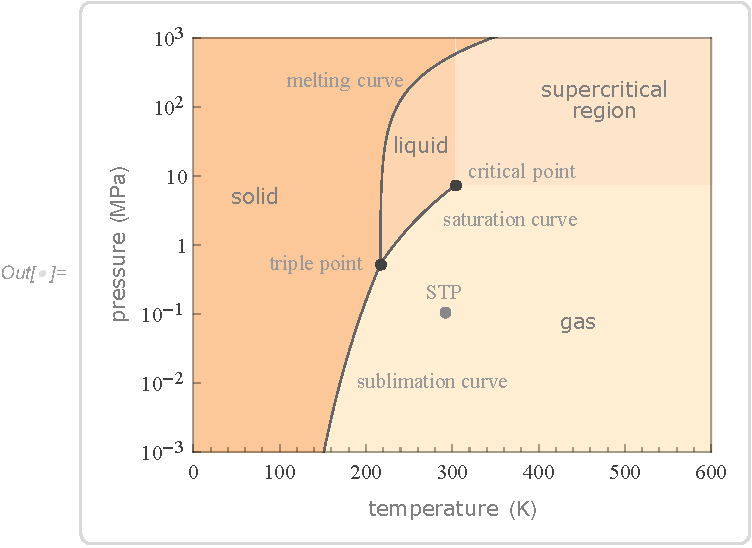
\includegraphics[width=\textwidth]{Figures/CO2PhaseDiagram}
\decoRule
\caption[The carbon dioxide phase diagram]{The phase diagram of carbon dioxide}
\label{fig:co2phase}
\end{figure}

The critical pressure of carbon dioxide is 304.12 K (31.10 °C) , and the
critical pressure is 7.39 MPa (72.9 atm). This temperature and pressure are easy
to achieve in the laboratory with standard chromatographic instrumentation, or
in an industrial plant with standard process engineering technologies.

Carbon dioxide is gaseous at ambient conditions. This means that once it has
been used in it's role as extractant, and it is exposed to the atmosphere, it
will rapidly evaporate, without needing added heat, and leaving no residues.

Any pure compound will have a supercritical point. Compounds with
technologically feasible supercritical points and useful chemical properties
include ammonia, methanol, CFCs/Freon, hydrocarbons (propane, butane), water and
sulfur hexafluoride. All of these lack green attributes: hyrocarbons pollute,
the CFCs deplete ozone, sulfur hexafluoride is a potent greenhouse gas, and
methanol and water are liquid at ambient conditions.

For these reasons the term supercritical fluid extraction is practically
synonymous with extraction using high-pressure carbon dioxide.

It is also possible to use supercritical fluids as reactants. This topic
falls outside the scope of this discussion.
 
\subsubsection{Modifiers}

\label{sec:modifiers}

The carbon dioxide molecule has zero dipole moment and the bulk fluid a low
dielectric constant, so supercritical carbon dioxide is expected to be
a non-polar solvent. (Although in practice the solvent behaviour is more
complex, partly explained by the high quadrupole moment of the carbon dioxide
molecule \autocite{Raveendran2005}.)

While the solvating power of a supercritical fluid is certainly `tuneable' by
adjusting its pressure and/or temperature, the range in solubility might be
quite limited in practice. Just as with other solvents, it is possible to add a
co-solvent or \textit{modifier} to the supercritical carbon dioxide. This makes
it possible to increase the solubility of polar compounds in the supercritical
fluid. Methanol, ethanol, formic acid, and water are examples of suitable green
modifiers for carbon dioxide \autocite{Herrero2010}.

When modifiers are used the carbon-dioxide, modifier and solute forms a system
with four degrees of freedom (modifier percentage, solute concentration,
pressure, and temperature), which can become difficult to model. While this is a
challenge for process engineers who need to design efficient industrial systems,
analytical chemists can afford to be pragmatic and use heuristics to find
suitable conditions \autocite{Wells2003}.

\subsubsection{Practical extractions}

Figure \ref{fig:sfediagram} shows a schematic diagram of a system set up for
supercritical fluid extractions.

\begin{figure}
\centering
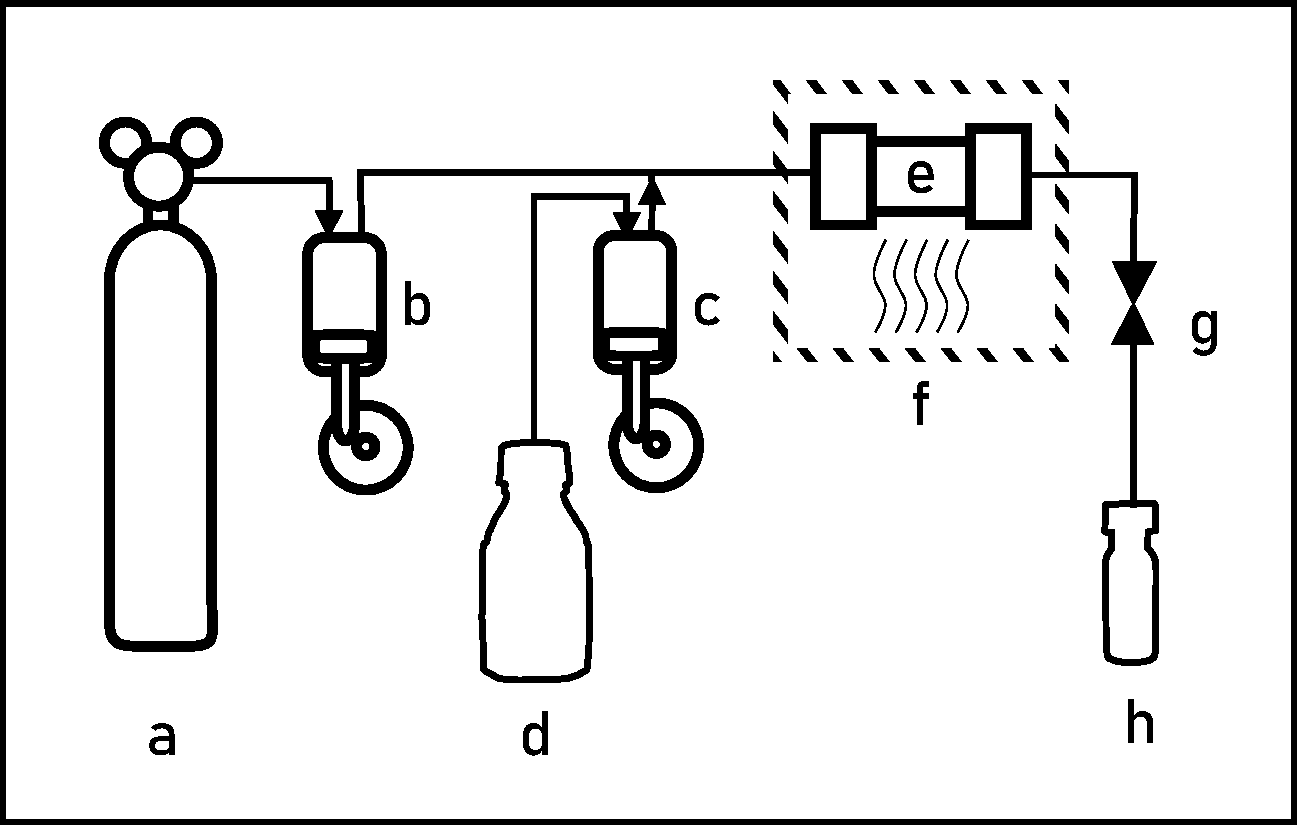
\includegraphics[width=\textwidth]{Figures/SFE_System}
\decoRule

\caption[SFE system diagram]{A diagram of an SFE system. (a) CO\textsubscript{2} supply (b)
High-pressure SF pump (c) High-pressure modifier pump (d) Modifier reservoir (e)
Extraction cell (f) Pressure control (g) Collection vessel}

\label{fig:sfediagram}
\end{figure}

Carbon dioxide (a) is readily available from suppliers of industrial gases, and
high-purity grades are available. Chromatography-grade solvents are usually used
as modifiers (d). High-pressure pumps (HPLC type) are used to compress the
carbon dioxide (b) and the modifier (c), which are mixed together at the
appropriate ratio. The mixture gets pumped into the (optionally heated (f))
extraction cell (e), which contains the material that needs to be extracted.
Having extracted the extract from the material, the supercritical fluid passes
through a pressure-control mechanism (g). This allows the pressure of the
supercritical fluid to drop to ambient, turning it into a low-density
non-solvating gas. The extract becomes desolvated, and precipitates in the
collection vessel (h). The operation of the system might be either static or
dynamic: in static operation the supercritical fluid is pumped into the system,
the flow is stopped, and the matrix/fluid mixture is given time to approach
equilibrium. Then the fluid is expelled and the extract collected.
In dynamic operation the supercritical fluid is pumped through the extraction
cell and the extract collected continuously. 


\section{Supercritical Fluid Chromatography}

An analyte will extract out of a matrix into a given solvent with a certain
efficiency and at a certain rate. While this is important while finding an
optimum extraction method, otherwise its relevance is limited.

However, \textit{different} analytes will extract out of a matrix with
\textit{different} efficiencies and at \textit{different} rates. In a 1906 paper
the Russian botanist Tsvet applied this observation to the dynamic extraction of
a bed of calcium carbonate that had mixture of plant pigments applied at the
inlet end, using petrochemical solvents. The different extraction efficiencies
and rates of adsorption and desorption on the calcium carbonate surface lead to
the \textit{separation} of the compounds in the mixture. Tsvet called this
method of separation \textit{chromatography} \autocite{Ettre1993,Ettre1993a}.
With time this method became generalized, and today chromatography is a major,
established scientific field with many ramifications and a myriad of
applications.

Because of the different technologies used in its applications, chromatography
is conventionally classed by the state of it's mobile phase as either
\textit{gas chromatography} (GC) or \textit{liquid chromatography} (LC).
However, as we have seen, solvating gases can also extract analytes from solid
stationary phases, and hence the term \textit{supercritical fluid
chromatography} (SFC) was created for these kinds of separations.

\begin{figure}
\centering
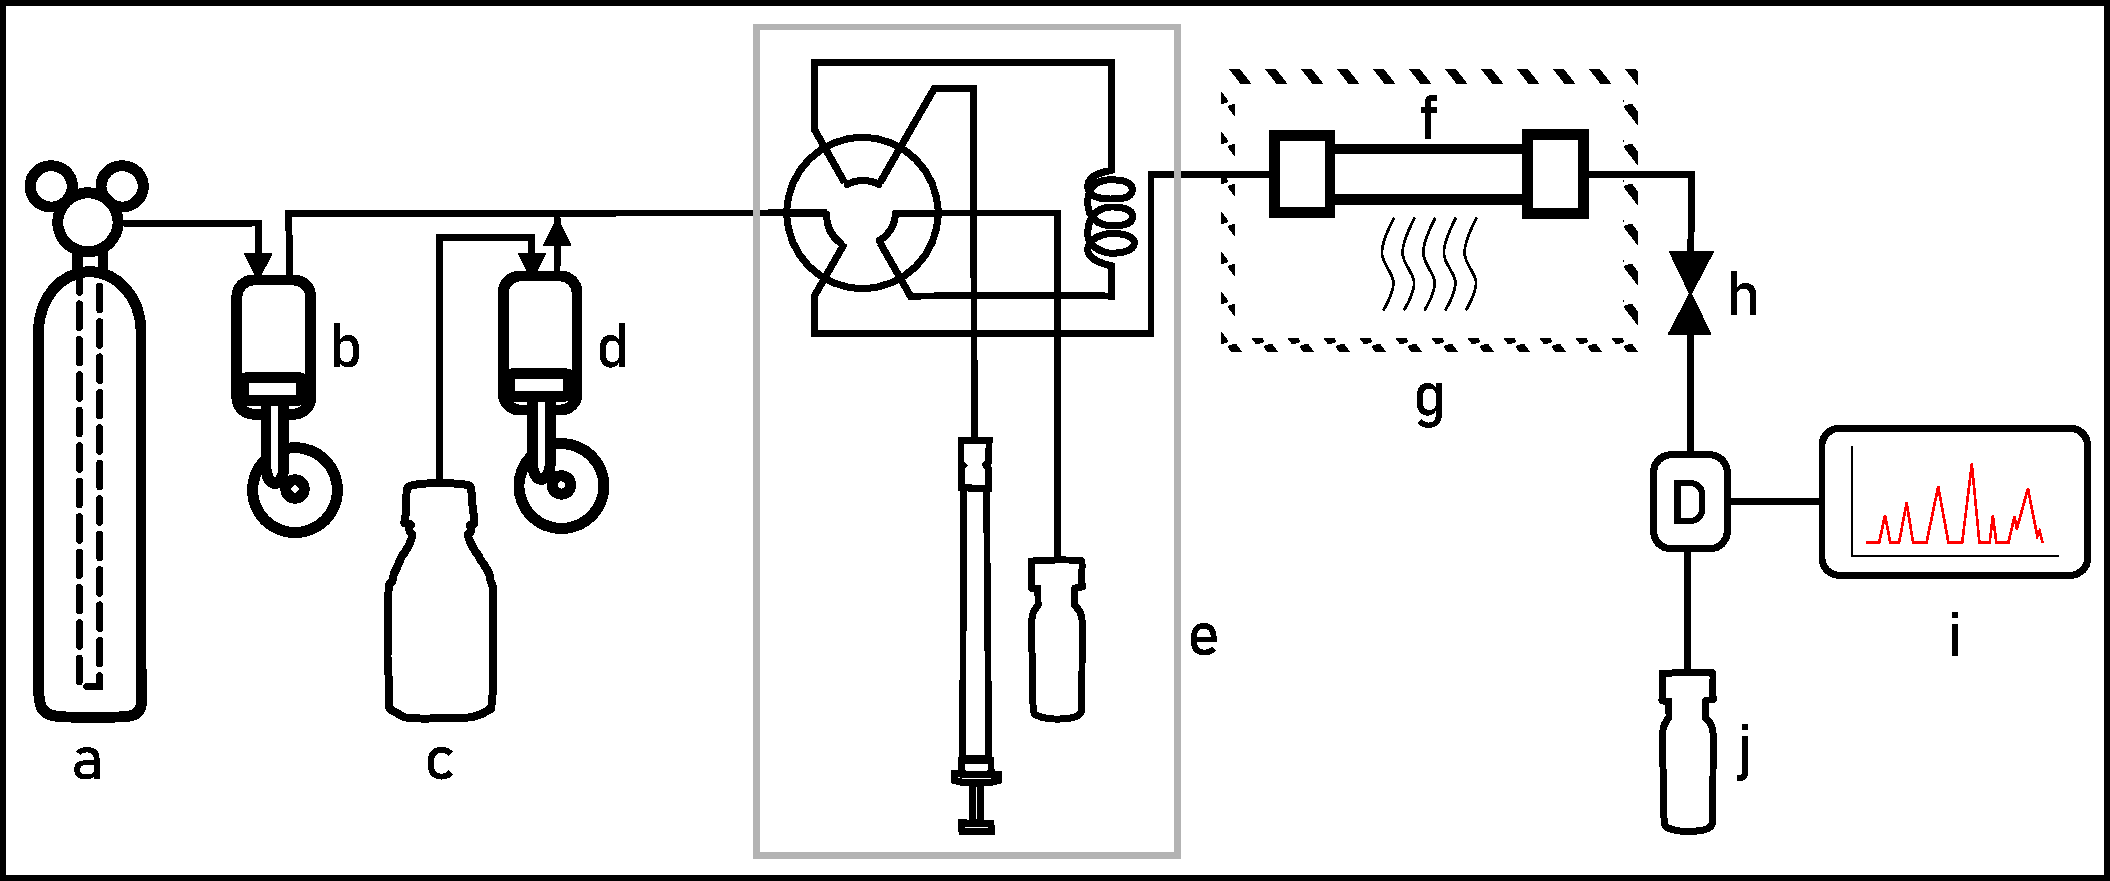
\includegraphics[width=\textwidth]{Figures/SFC_System}
\decoRule
\caption[SFC system diagram]{A diagram of an SFC system. (a) CO\textsubscript{2}
supply (b) High-pressure SF pump (c) Modifier reservoir (d) High-pressure
modifier pump (e) Injection system (f) Column (g) Optional heating (h)
Back-pressure control (D) Detector (i) Data system (j) Optional fraction
collection.}
\label{fig:sfcdiagram}

\end{figure}

Supercritical fluid chromatography as practised today bears a great resemblance
to \textit{high performance liquid chromatography} (HPLC). The main reason for
this is that there is a large overlap between the technology used for HPLC and
the technology needed for SFC. In particular, both use high-pressure pumps and
columns packed with particles of very small diameter, and use optical
detectors. The same instrument manufacturers who supply HPLC instrumentation
also supply SFC instrumentation.

\subsection{SFC and FID}

But SFC was not always a technique based on HPLC technology. In the 1980s SFC
was practised using open tubular columns and flame detectors, so the instrument
designs looked more like GC instruments than HPLC instruments, and SFC was sold
as a replacement for GC \autocite{Poole2003}.

During this era the detectors used for SFC was the flame-based detectors used
for CG, in particular the flame ionization detector (FID).

The \textit{flame ionization detector} was invented near-simultaneously in South
Africa and New Zealand \autocite{Ettre2008}. The core of the system is a
flame of hydrogen gas burning in pure air. The measured signal is the conductivity of
the flame plasma, which is measured by applying a {-100} V potential difference
between electrodes at the tip and the base of the flame. There are very few free
ions in the hydrogen flame, so the conductivity is normally low. But organic
compounds introduced into the flame creates a number of free ions, which
increases the conductivity of the flame gases. The change in conductivity is
measured by measuring the current between the two electrodes, using an electrometer. 

As a first approximation the signal produced by the FID is proportional to the
number of carbon atoms in the analyte. This is rather surprising, until the
mechanism of its working is elucidated. At high temperature in the hydrogen-rich
core of the flame, all hydrocarbon atoms are reduced to methane
\autocite{Holm1996}. Once it gets into contact with the hot oxygen in the outer
layers of the flame there is a chemi-ionization reaction. The electric field
acting on the ions creates a flow of ions, which can be measured as an electric
current.

\begin{figure}
\centering
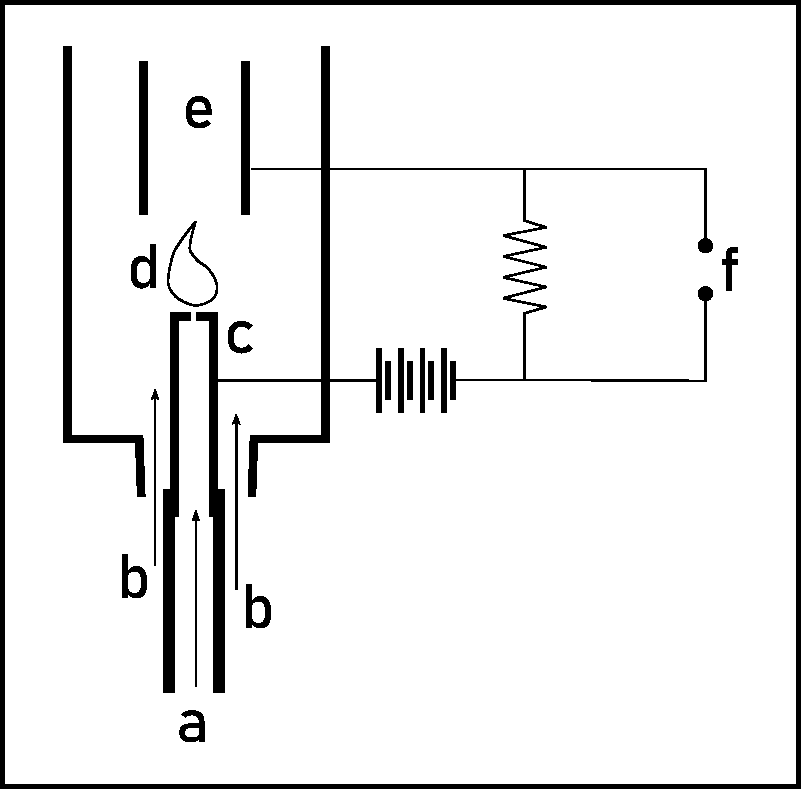
\includegraphics[width=\textwidth]{Figures/FIDSchematic.pdf}
\decoRule

\caption[FID diagram]{A schematic diagram of the flame ionization detector. (a)
Mixture of column eluate and hydrogen gas (b) Clean air (c) Metallic flame tip
electrode (d) Collector electrode (e) Conductivity signal}

\label{fig:fiddiagram}

\end{figure}

The FID's shining strength as a detector is its tremendous linear dynamic range
of 10\textsuperscript{7}. Combining the linear dynamic range with its carbon
sensitivity makes it an excellent detector for quantifying organic compounds.

During period of history that SFC was seen as a variant of GC, the FID was the
detector of choice. But when SFC started looking like HPLC, and the selectivity
of the chromatography started being manipulated by adding modifiers (see Section
\ref{sec:modifiers}), the FID lost its utility. The quantity of modifier added
to the carbon dioxide mobile phase swamps the FID detector, making it useless as
a detector. In contrast, if the chosen modifiers are transparent at the relevant
wavelengths, optical detectors are more useful in SFC using modified carbon
dioxide as a mobile phase.

\subsection{SFC×GC}
\label{sec:SFCxGC}
In chromatography, the analyte in the eluate can be detected to yield
information about the sample, or fractions of eluate can be collected for
further purification or characterization, or both. If fractions are collected,
there is nothing that prevents the chromatographer from subjecting a collected
fraction to another chromatographic separation.

For example, a synthetic chemist might use column chromatography to separate
their target compound from side-reaction compounds, collecting fractions of the
eluant. If the compounds are colourless, the chemist might use
\textit{thin-layer chromatography} (TLC) to examine the fractions for presence
and purity of the relevant compounds.

If the product and the side-product were co-eluting it would not help to use the
same chromatographic system (\textit{i.e.} combination of stationary phase and
mobile phase) for the TLC examination, because the co-elution would not become
apparent. If, however, the chemist changed the mobile phase, or switched to a
different stationary phase for the TLC examination, then it is quite likely that
the two compounds would be separated. 

For example, if a synthesis involving sugars were being attempted, two sugar
enantiomers would likely co-elute on a silica clean-up column. Investigating the
sugar fraction using a TLC plate with a chiral stationary phase
would reveal the presence of stereoisomers.

The second, chiral separation (on TLC) is said to be \textit{orthogonal} to the
first (packed column) separation.

Such a separation is an example of a two-dimensional (2D) separation. In
analytical chromatography, 2D separations are powerful tools.

The simplest 2D chromatography is called \textit{heart-cutting}. In such a case
a fraction of interest is collected from the first dimension
(\textsuperscript{1}D) separation, and subjected to a second dimension
(\textsuperscript{2}D) separation. For example, a fraction collected from an
HPLC separation could be injected into a gas chromatograph. The separation on
the GC dimension would obviously be very different from the separation on the
HPLC dimension, and therefore we can say that the orthogonality is high.

Heart-cutting is a useful way to get detailed information from a sample, but it
is technically demanding and labour-intensive. It is usually employed for
challenging separations in well-understood samples, because peaks of interest
in the first dimension must be captured for injection on the second dimension.

If, however, one collects the eluate in equal fractions and do identical
separations on each of the fractions, then one enters the domain of
\keyword{comprehensively coupled chromatography}. The comprehensive coupling of
orthogonal chromatographies does not demand a previous understanding of the
sample, and doing exactly the same separation for each fraction allows the
process to be automated.

A 2D separation can be called comprehensive if the following three criteria are
met \autocite{Giddings1987}:

\begin{enumerate}
  \item Every part of the sample is separated by two distinct chromatographic processes.
  \item Equal percentages of all sample fractions are separated by the second process.	 
  \item Compounds resolved by the first dimension separation remains resolved.  
\end{enumerate} 

To effectively distinguish between heart-cut and comprehensive 2D couplings, a
terse nomenclature was developed. Simple coupling between systems is
designated by a hyphen (``-''), for example HPLC-GC. This corresponds to the
usual notation of a coupled detector coupled to a chromatograph, for example
GC-FID or GC-MS. Comprehensive coupling is denoted by a multiplex sign
(``$\times$''), for example GC$\times$GC. If it is not clear from the context,
the detector can be specified using a hyphen, as in GC$\times$GC-MS.

Of the comprehensive coupled chromatography techniques, GC$\times$GC is the most
mature, with a selection of powerful instruments on the market.

This thesis further explores the implementation of SFC$\times$GC, as first
developed by Venter and Rohwer \autocite{Venter2004, Venter2006}.

In this implementation of SFC$\times$GC, fractions of the eluate of the SFC is
transferred to the GC. The mobile phase is changed from carbon dioxide to
hydrogen in the modulating interface, and the GC dimension is a conventional open-tubular
capillary separation with FID detection.

Any volatile modifiers or additives added to the SFC mobile phase will be separated from
the analytes by the GC dimension. This makes in possible to use the FID as a detector
in an SFC$\times$GC chromatograph where the SFC is based on HPCL technology.

The \textsuperscript{2}D separations are \textit{fast} chromatographic
separations, \textit{i.e.} separations optimized for speed, sacrificing
resolution. This is achieved using fast temperature programming of the GC
separation.

The high orhtogonality of the SFC and the GC separations enables novel comprehensive 2D
chromatography, which we applied to the chemical analysis of biodiesel.
